\documentclass[authoryear, 12pt,5p, times]{elsarticle}
%\usepackage[hypcap]{caption}
%\geometry{margin=0.95in,top=1.4in,bottom=1.4in}
\geometry{margin=1in,top=1.3in,bottom=1.3in}
\usepackage{float}
\usepackage{amsmath}
\usepackage[hidelinks]{hyperref} 
 \usepackage{gensymb}
\usepackage{subcaption}
\usepackage{url}
%\renewcommand\thefootnote{\fnsymbol{\dagger}}
\usepackage[symbol*]{footmisc}
\makeatletter
\newcommand{\rpm}{\raisebox{.3ex}{$\scriptstyle\pm$}}
\begin{document}
%\footnote{This is a footnote}
\begin{frontmatter}
\title{Doppler Measurement of Solar Rotation}
\author{\today \\ \quad \\Jung Lin (Doris) Lee\\ dorislee@berkeley.edu\\Group partners: Jennifer Ito, Manuel Silvia\\Prof. James Graham, UGSI Heechan Yuk, Isaac Domagalski}
	\begin{abstract}
In this experiment,  we------
we use the method of least squares to calibrate the wavelength calibration 
	\end{abstract}
\end{frontmatter}
\section{Introduction}
\section{Data Reduction}
\subsection{Dark, Bias, Flat Subtraction}
\label{subtraction}
Using the halogen lamp as a source of uniform illumination, the flat field images calibrate the pixel-by-pixel variations as well as common artifacts that is seen in both continuum sources as shown in Fig. \ref{calib}. We take the ``dark frame" as the the average of the ---- (i.e. the flat region shown in Fig. ----) before and after the  . Without subtracting the bias in the ``dark image", we can automatically get bias subtraction by simply subtraction off the dark, as the bias is incorporated as part of the ``dark frame" .
Every image pixel is:
\begin{equation}
			\frac{\text{image}-\text{dark}}{\text{flat}}\times\text{median(flat)}
			\label{calib_eq}
\end{equation}
 \begin{figure}[h!]
 When converting the 2D images to 1D spectra, we took a 1024-by-1024 pixel slice of the image array to truncate the 24 overscan pixels.
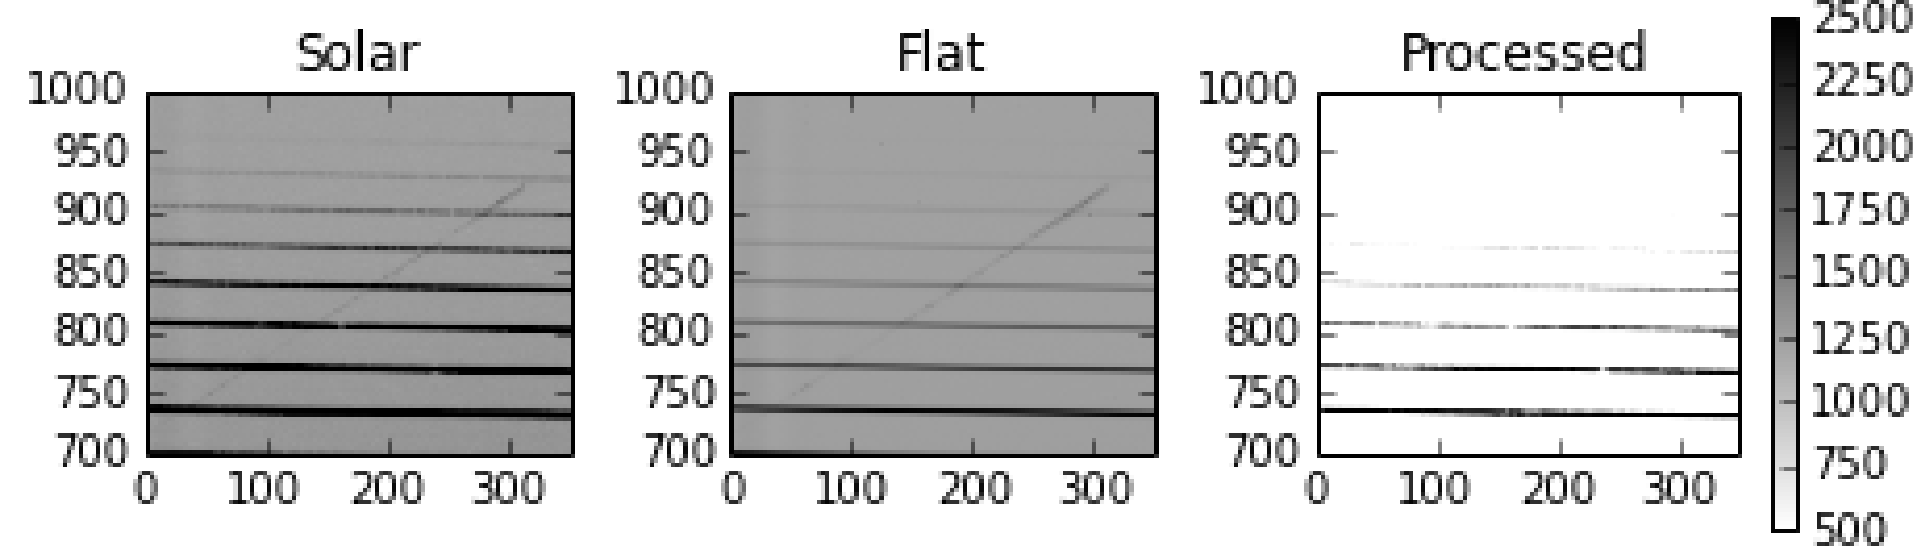
\includegraphics[width=0.5\textwidth]{figures/processed}
\caption{Both continuous sources shows the same artifact in a corner of the CCD image. The figures below are zoomed in --- on this feature, which  possibly from the reflected light . The halogen exposure is used for flat correction. Along with subtracting the background from the non-incident solar spectrum, the artifact is removed in the proceessed image shown in the rightmost figure.}
\label{processed}
\end{figure}
\subsection{Spectrometer details}
The spectrometer consists of a 300 mm$^{-1}$ transmission grating that disperses the collimated incident beam and a 80 mm${^-1}$ echelle grating 
 perpendicular to it. The resulting image captured by the APOGEE 13 $\mu$m CCD is a 1024 $\times$ 1024 image array with different orders of diffraction projected as a row spanning 20nm across. 
\hspace{-20pt}
\begin{table}
    \begin{tabular}{|l|l}
%    \hline
    \hline Angular dispersion [$m^{-1}$]  & 4.804                     \\ \hline     \hline Free spectral range [nm]           & 18.16                     \\     \hline Min wavelength [nm]  & 625.6
 \\  \hline  Max wavelength [nm]  &  643.76 
 \\ \hline Magnification   & 0.3357                
 \\ \hline  \hline     Angular dispersion [$m^{-1}$]  & 4.804                   \\ \hline   Spectral resolving power  & $1.317\times10^4$\\ 
    \hline Spectral resolution [km/s]   & 54.09        \\ 
   \hline Width on the CCD [mm]   & 0.52                      \\
    \end{tabular}
  
    \caption{Computed spectrometer information for $\lambda $=632.8 nm, corresponding to echelle order of  m=35. }
  \label{spec_prop}\end{table}
 \\The spectral resolution in nm deals with the distance between two closely spaced features so that the features are resolved. This quantity can be computed by Eq.\label{spectral_resolution}
\begin{equation}
\delta\lambda=\Bigg(\frac{\partial\lambda}{\partial\beta}\Bigg)_{m,\alpha}\Bigg(\frac{\partial\beta}{\partial\alpha}\Bigg)_{m,\lambda}\delta\alpha
\label{spectral_resolution}
\end{equation}
where $\Big(\frac{\partial\lambda}{\partial\beta}\Big)_{m,\alpha}$ is the reciprocal of the angular dispersion and $\Big(\frac{\partial\beta}{\partial\alpha}\Big)_{m,\lambda}$ is the anamorphic magnification computed as a ratio of the cosines of the incident and diffraction angles. The numerical result for the m=35 order is 3.629 pixels. Using the dispersion relation for pixel-to-wavelength conversion and the Doppler velocity formula described by Eq.\ref{doppler_eq}, we determine the resolution for the velocity measurement in km/s as cited in Table.\ref{spec_prop}.
\\
\begin{figure}[h!]
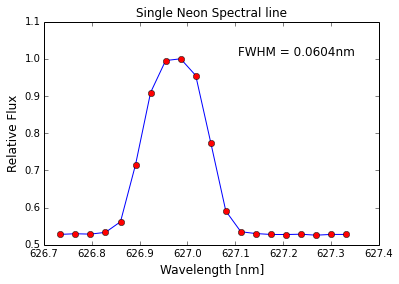
\includegraphics[width=0.5\textwidth]{figures/single_neon}
\caption{Above figure shows a single neon emission line. Since intensity distribution follows a normal distribution, the FWHM is computed by 2$\sigma\sqrt{2\ln(2)}$ where $\sigma$ is the standard deviation of cropped image containing a single neon line. Just like $\sigma$, the FWHM informs us about the width of a distribution. }
\label{lambda_direction}
\end{figure}
\subsection{Wavelength Calibration}
From the halogen spectrum we deduced that the cross-dispersion wavelength ( $\lambda_{cd}$) decreases along the direction of y axis and from the tilted order, we conclude that the wavelength from the echelle grating ($\lambda_{e}$) increase from right to left.
We took exposures where both the neon light and 635nm green laser was turned on in order to identify  where ----- .Since each order has a slightly different coefficient, we chose to calibrate the order containing the 635nm green laser. as a convient 
\begin{figure}[h!]
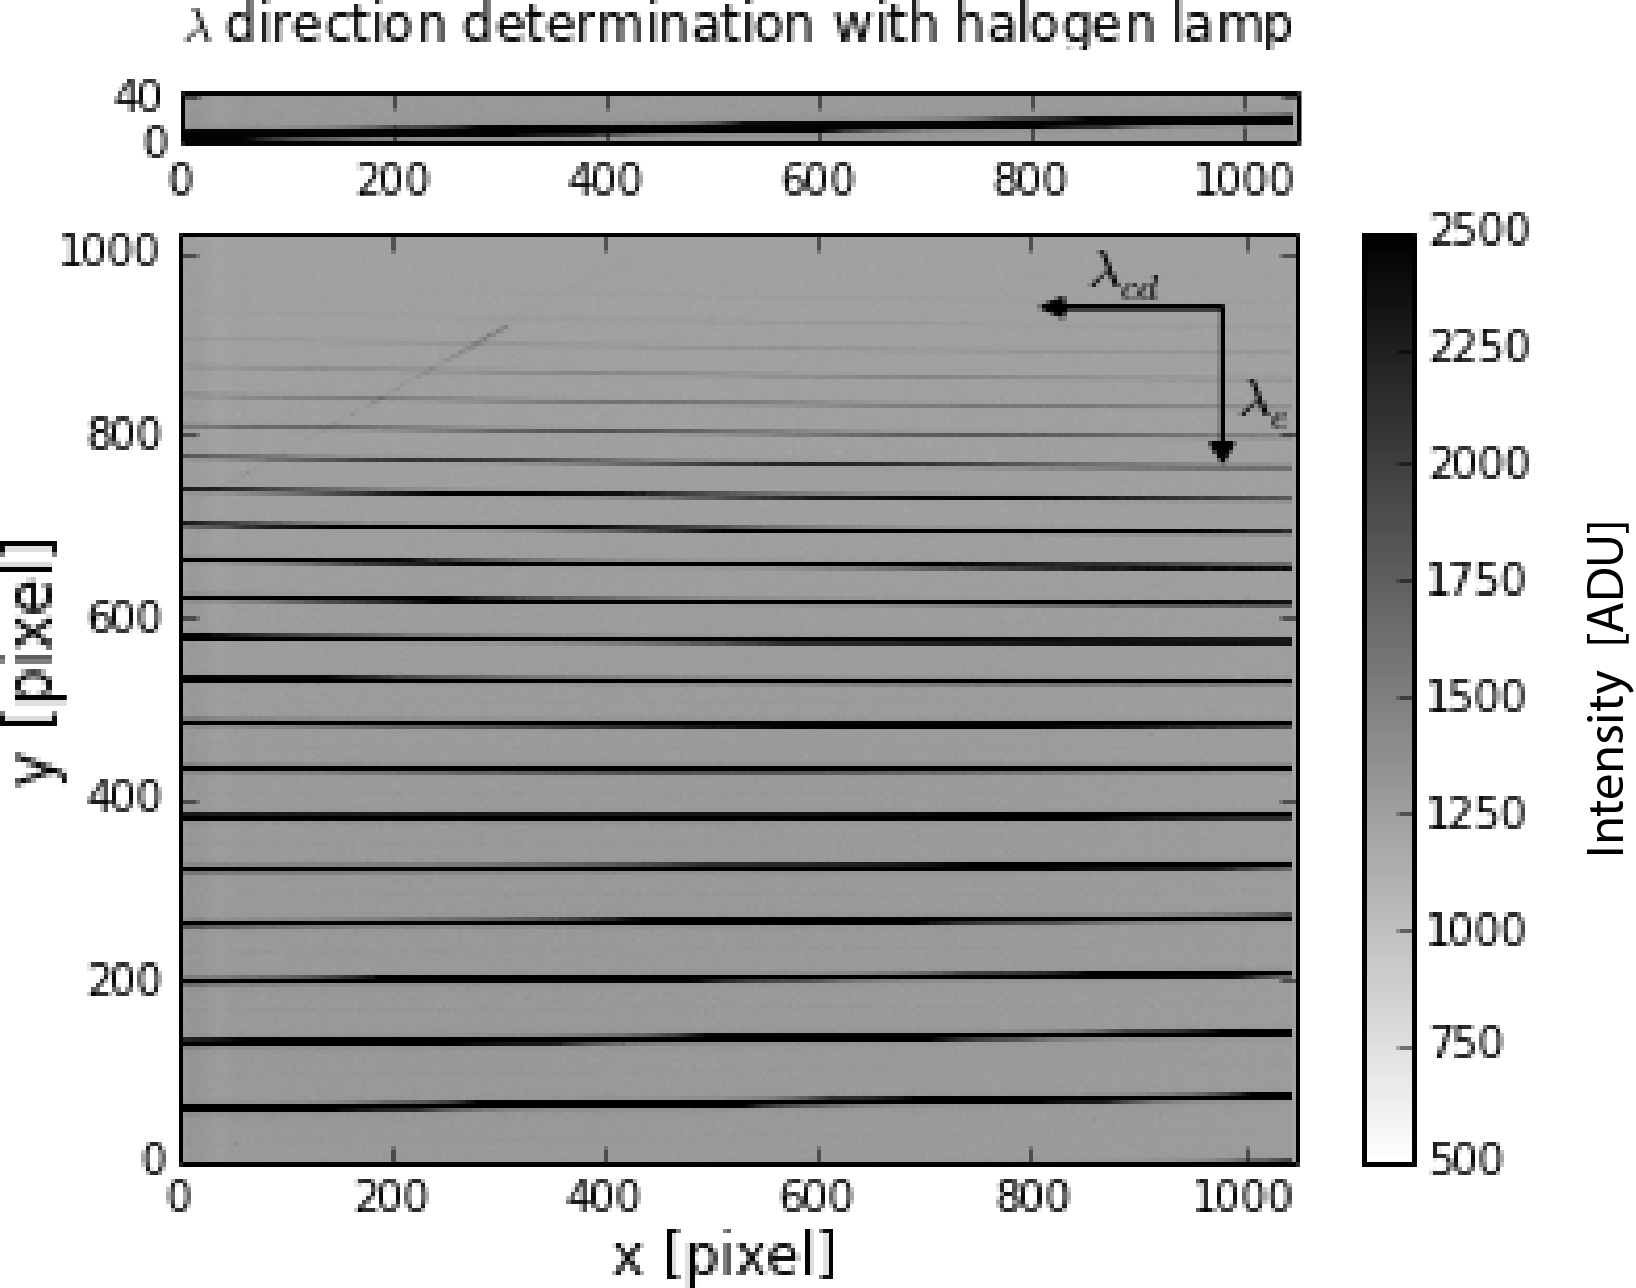
\includegraphics[width=0.5\textwidth]{figures/lambda_direction}
\caption{Wavelength direction, the arrow points in the direction of increasing wavelength. We determine the tilting direction from a zoomed-in section of a single echelle  order, as shown in the top figure.}
\label{lambda_direction}
\end{figure}
 \begin{figure}[h!]
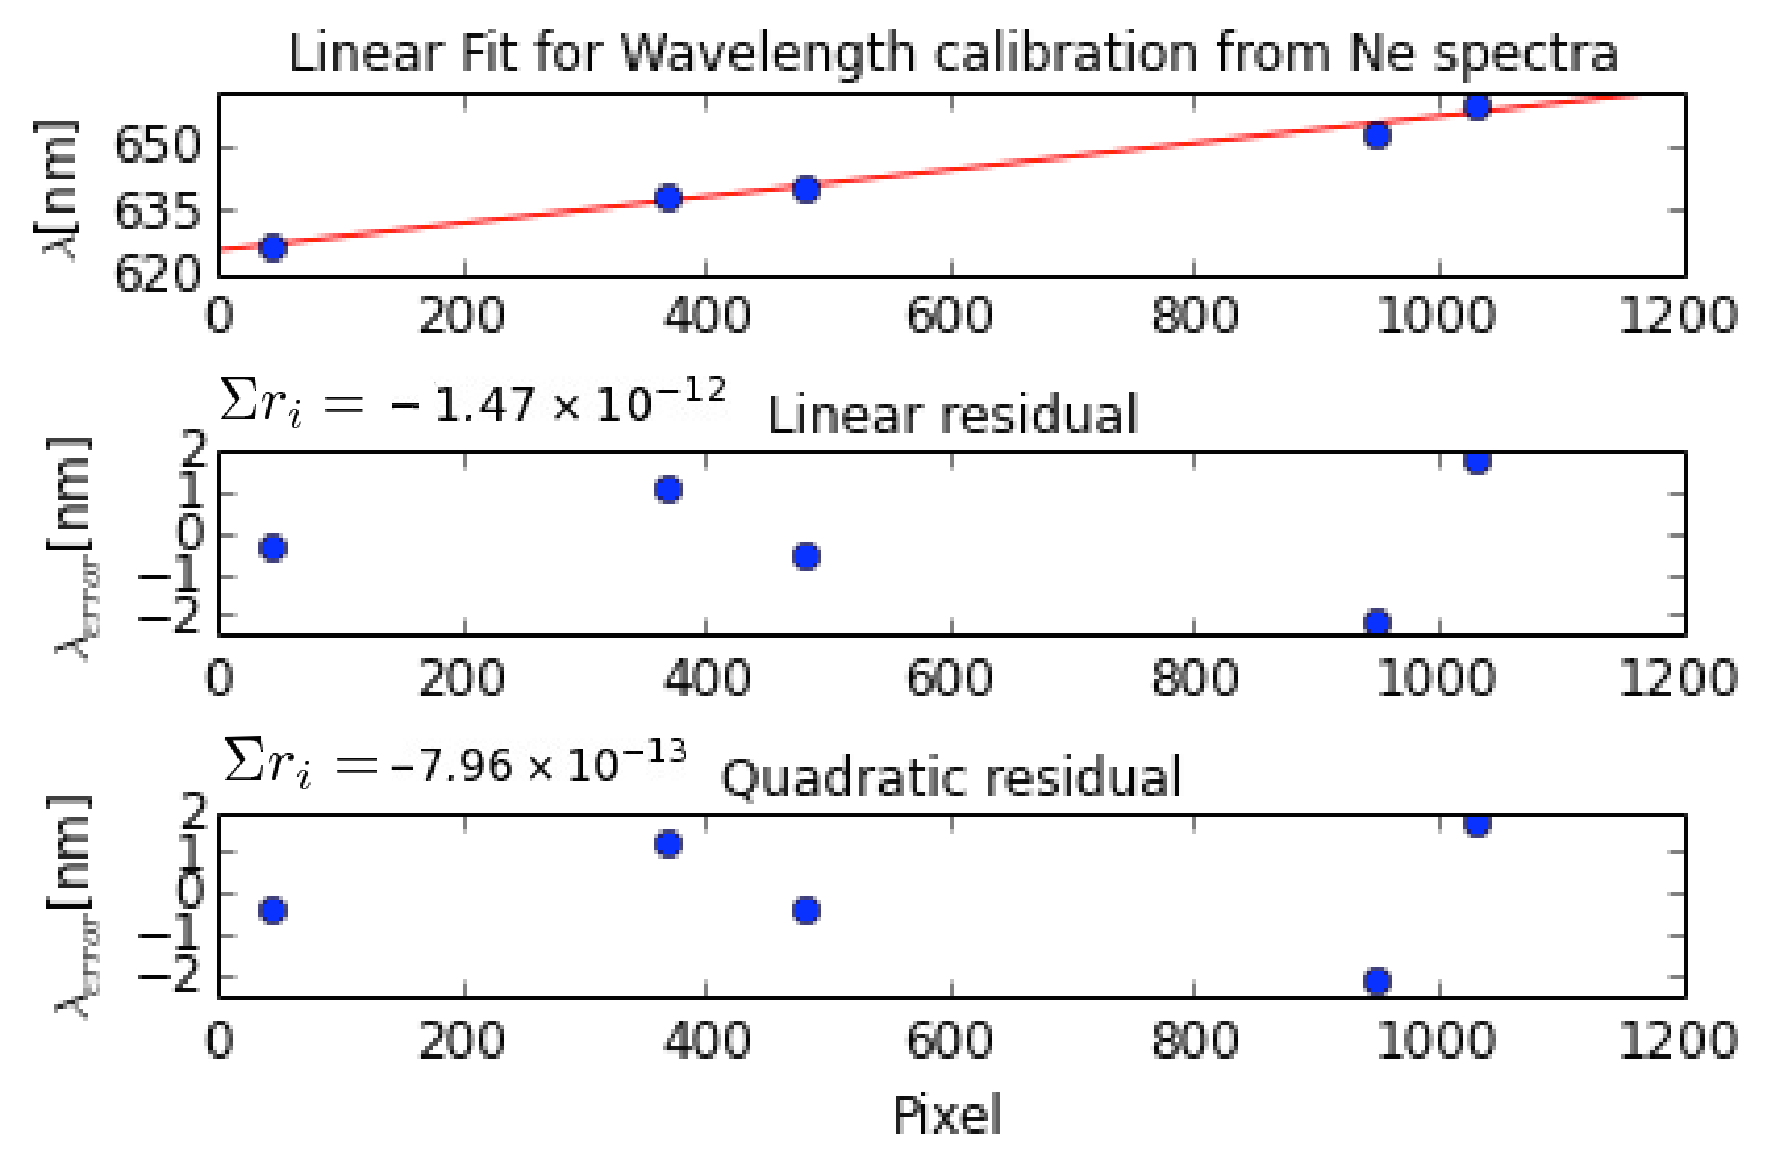
\includegraphics[width=0.5\textwidth]{figures/wavelength_calib}
\caption{The first order fit in the top figure shows that the dispersion is approximately linear ($\frac{d\lambda}{d\text{pixel}}$=0.0315 nm/pixel ). Since there is no notable patterns in linear residual and the magnitude of the residual is small, a linear relationship should be sufficient for pixel-to-wavelength conversion. From the bottom most quadratic figure, we see that the residual decrease by an order of magnitude.}
\label{calib}
\end{figure}
\subsection{Limb Darkening}
The data quality of the solar scan can be verified by the a time series plot as shown in Fig. \ref{eddington_fit}. Intensity fluctuation that deviates from the predicted effect of limb darkening indicates possible shading effect from presence of cloud or objects near the telescope such as a crossing observer. Qualitatively, this information can be used to visually reject entire shaded scans or pick out exposures in the bright central region for a more accurate Doppler shift determination. Quantitatively, we can also make use of the limb darkening effect to determine crossing time of the solar scan, used in our solar angular size calculation in Sec.\ref{size_calc}.
\\
To avoid the arbitrary determination of the exposure that defines the start and end of the solar crossing, we fit our data to Eq.\ref{eddington_eq} with the center-to-limb time ($\Delta t$) as our varying parameter.  The lower figure in Fig.\ref{eddington_fit} shows the result of substituting the value of $\Delta t$ back into Eq.\ref{eddington_eq}, and ignoring the uneven data points on the two sides  (an artifact of the telescope) and the region before and after the solar crossing. Without this procedure, the fit would be largely distorted by the telescope artifact on the two sides and the ``dark" regions, which is not part of the stellar model.  Note that, the fit in Fig.\ref{eddington_fit} also does not fully include the first two scans after the jump, yielding a more accurate estimate for the crossing time. This way of defining the boundaries of the stellar atmosphere is a more robust method than simply selecting the datapoint where the jump in intensity occurs and computing $\Delta t$ from the FITS header time information.
\\
We see the effect of limb darkening by summing together the intensity of all pixel in every CCD image in a full solar scan. Limb darkening results from the limitation that an observer can only see into a constant optical depth of 2/3. As the density and temperature of a star decreases radially outwards, the observer sees light originating from different regions of the star corresponding to the darkening effect. The time series data in Fig.\ref{eddington_fit} shows the total intensity of each exposure scaled by the intensity at the central bright peak ($I_0$) which we set at the origin. By modelling intensity as a function of the incident viewing angle using the Eddington approximation for grey, plane-parallel stellar atmosphere, we obtain the relation: 
\begin{equation}
\frac{I(\theta)}{I(\theta=0)}=\frac{I}{I_0}= \frac{2}{5}+\frac{3}{5}cos\theta
\label{eddington_eq}
\end{equation}
By geometrically relating this with the Earth-sun distance and crossing times, we get: 
\begin{equation}
\cos \theta = \sqrt{1-(t-t_0)^2/\Delta t^2} 
\end{equation}
where $t_0$ is where the time of the central bright peak, t is the time of each scan and $\Delta t$ is the crossing time.
\begin{figure}[h!]
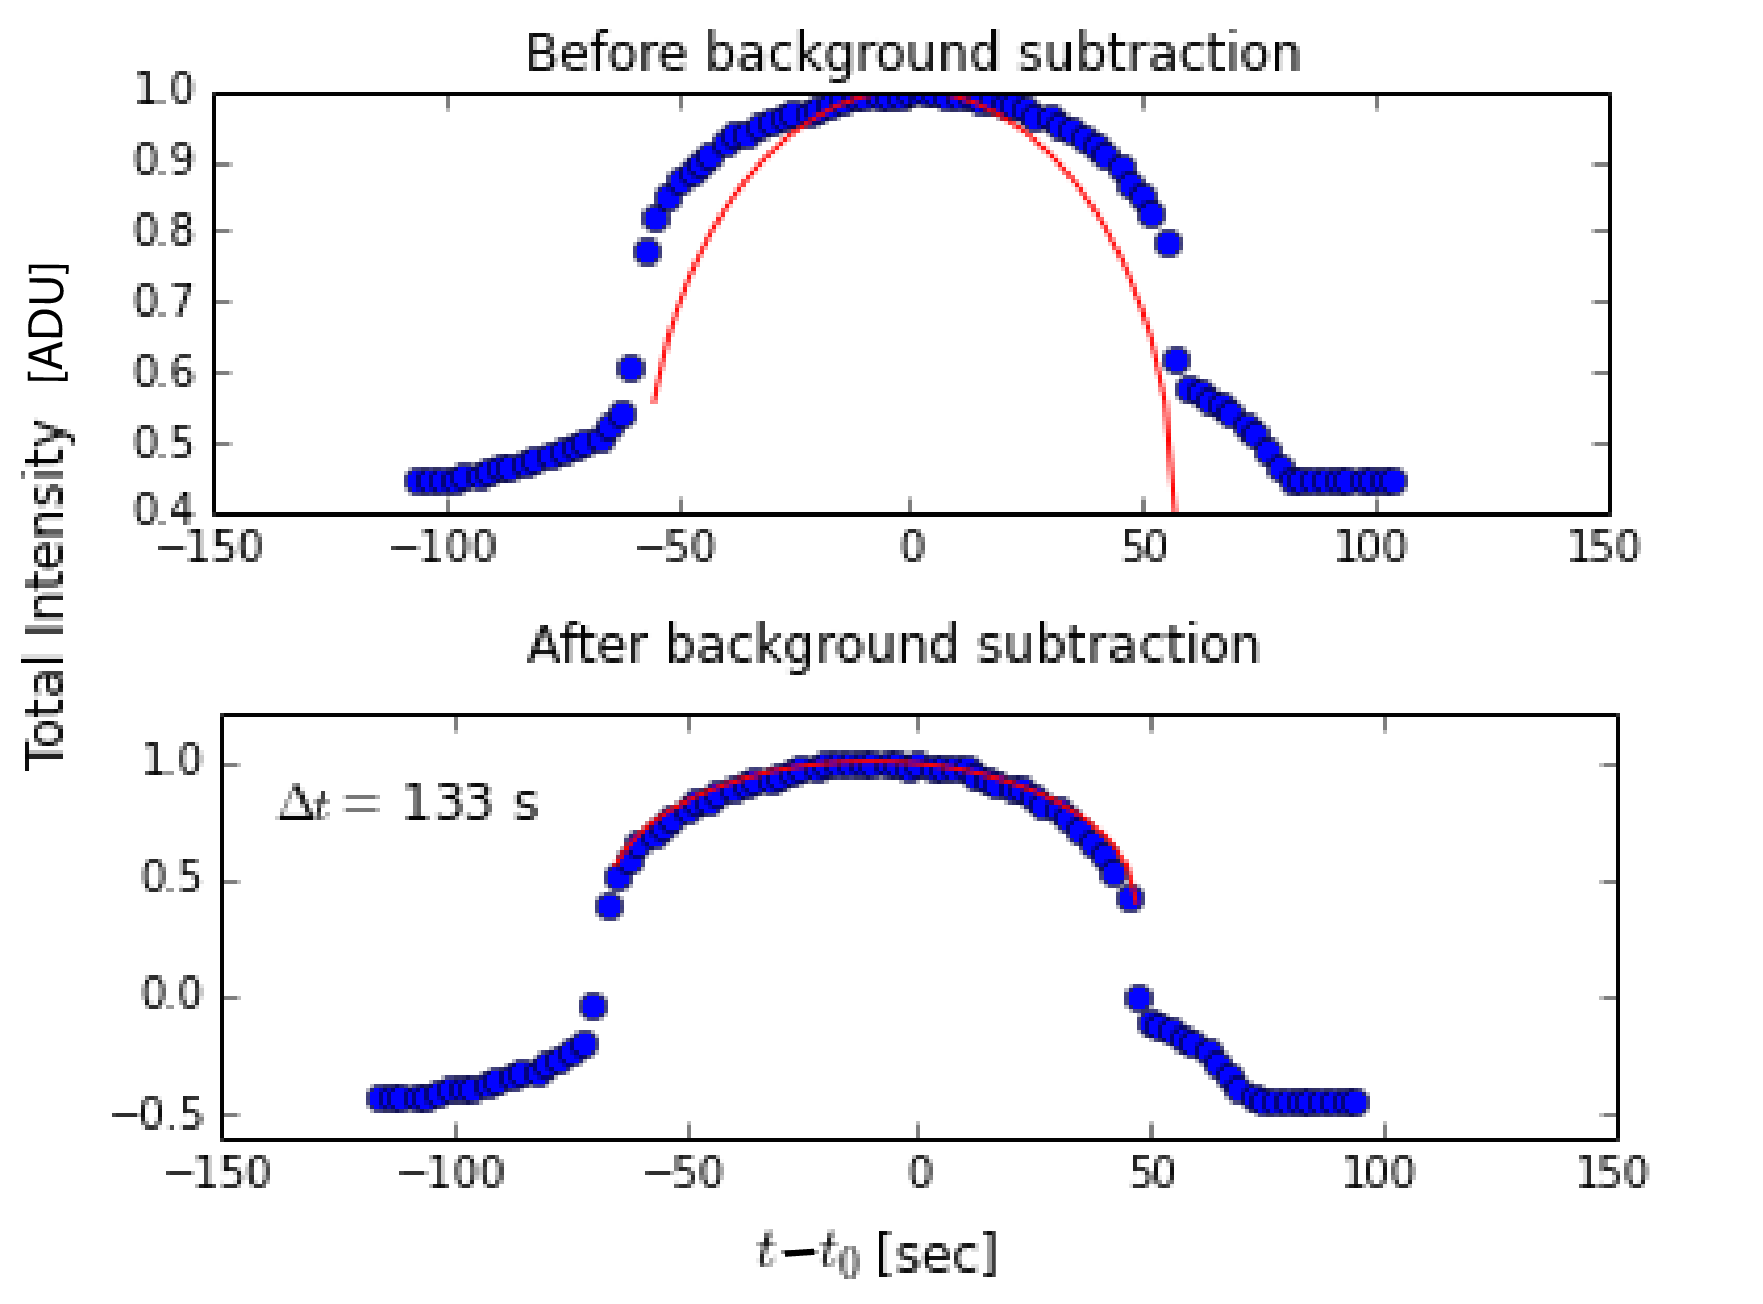
\includegraphics[width=0.5\textwidth]{figures/eddington_fit}
\caption{ The y-axis is normalized so that curve fitting corresponds to the model's output I/$I_0$ . The clear improvement of the model fit after background subtraction is evident as some of the intensity fluctuation may be mitigated by systematic effects corrected in the dark and flat frames discussed in Sec.\ref{subtraction}.}
\label{eddington_fit}
\end{figure}
\subsection{Cross-Correlation Analysis}
\begin{figure}[h!]
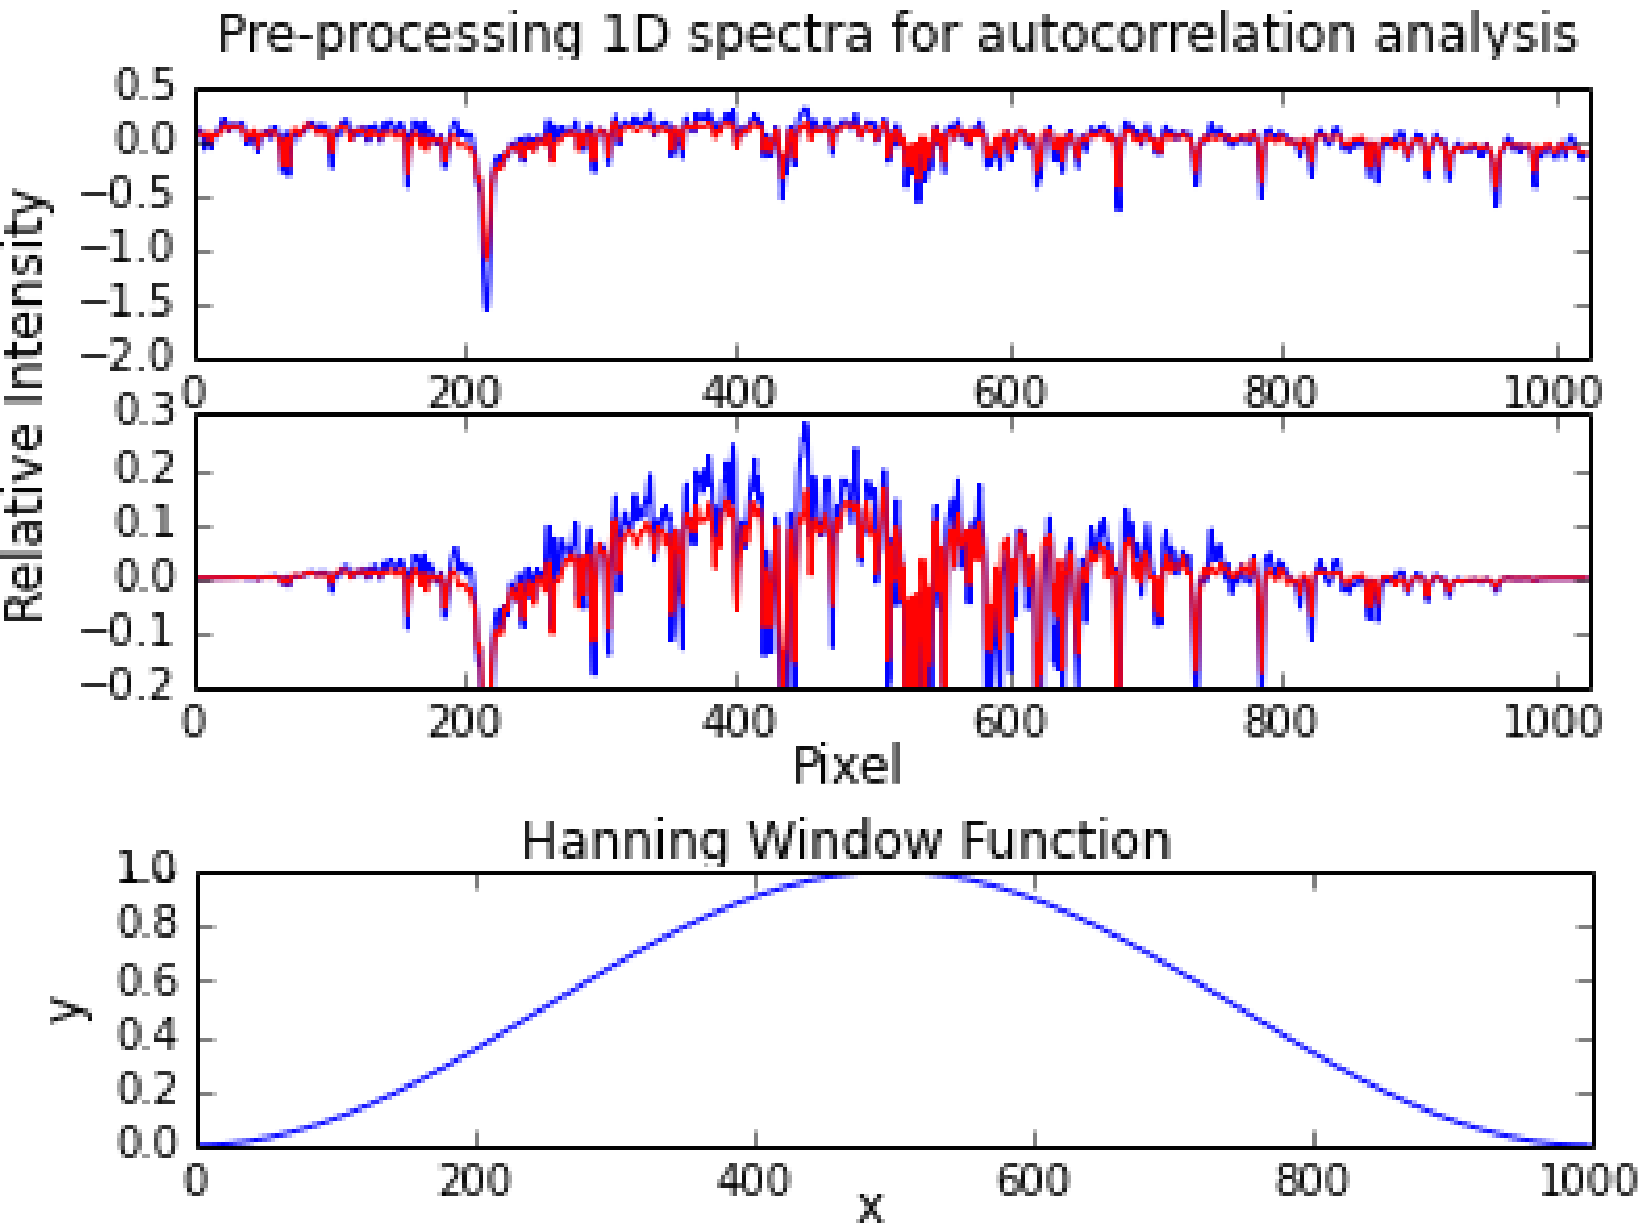
\includegraphics[width=0.5\textwidth]{figures/process_corr_spectra}
The cross correlation analysis is conducted by repeatedly trying different values of pixel lag to shift the a set of spectra and then computing its cross-correlation value with the ------  using Eq.\ref{autocovariance} 
\begin{equation}
s_j = \frac{1}{N-1}\Sum\lim_i \Big(x_i y_{i+j}\Big)-\frac{N}{N-1}(\bar{x}\bar(y))
\label{autocovariance}
\end{equation}
where $x_i$ is the 1D spectra
    ac = 1./(N-1)*sum(xi*xij)-N/float(N-1)*mean(xi)**2
\caption{Since we are measuring fractional pixel shift, process our data to make ---- more precise ( ?) . 
First, we subtract off the mean of the spectra so that all there is left is the deviation from the mean. This procedure preserves the shape of the peaks  but subtract out the ----- that exist in both datasets. Then, we multiply the resulting spectra by the Hanning window function (Bottom figure). Since the probability density function is normalized to one, the resulting spectra as shown in the middle figure is weighted by the window function. The weighing serves to put more emphasis on the data in the central region and ----- edge effect .   ----We have also tried doing this for .we average all the spectra in the solar scan }
\label{process_corr_spectra}
\end{figure}
\begin{figure}[h!]
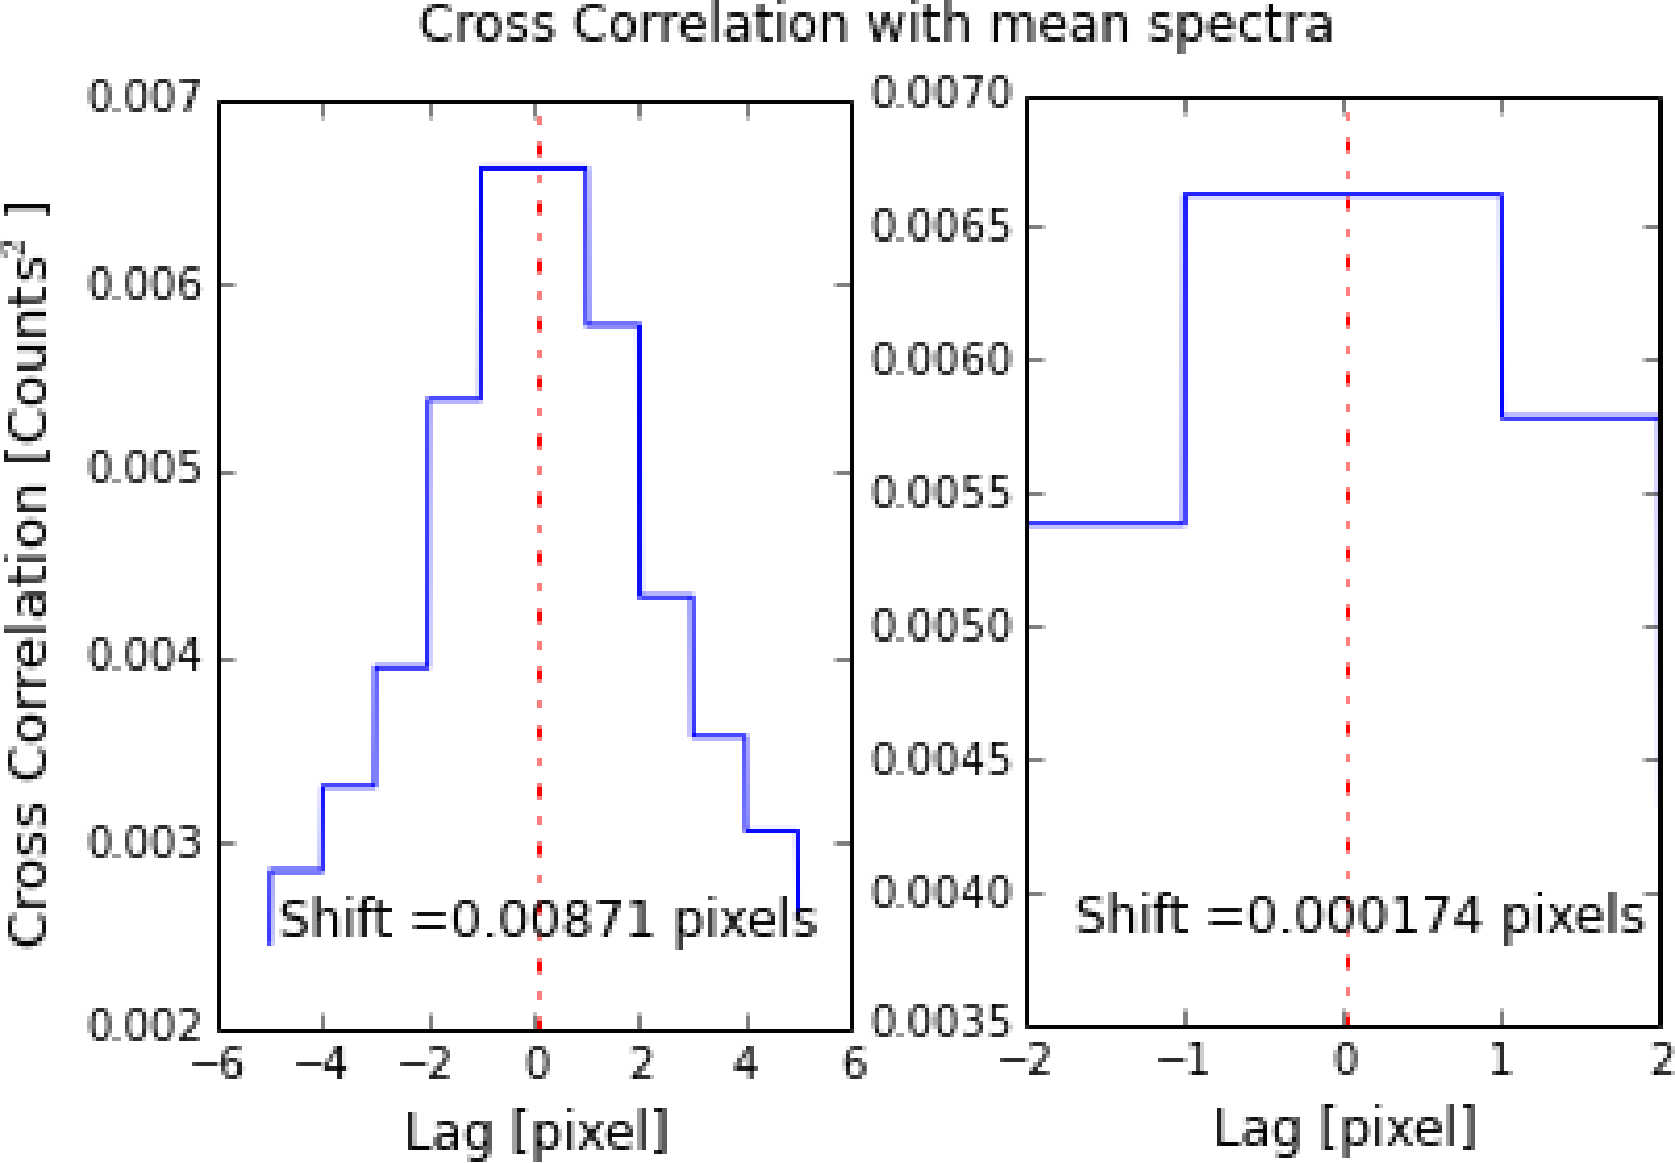
\includegraphics[width=0.5\textwidth]{figures/autocorr_curve}
\caption{}
\label{autocorr_curve}
\end{figure}
\begin{equation}
\delta\lambda=\frac{v}{c}\lambda_0
\label{doppler_eq}
\end{equation}
\section{Results}
\begin{figure}[h!]
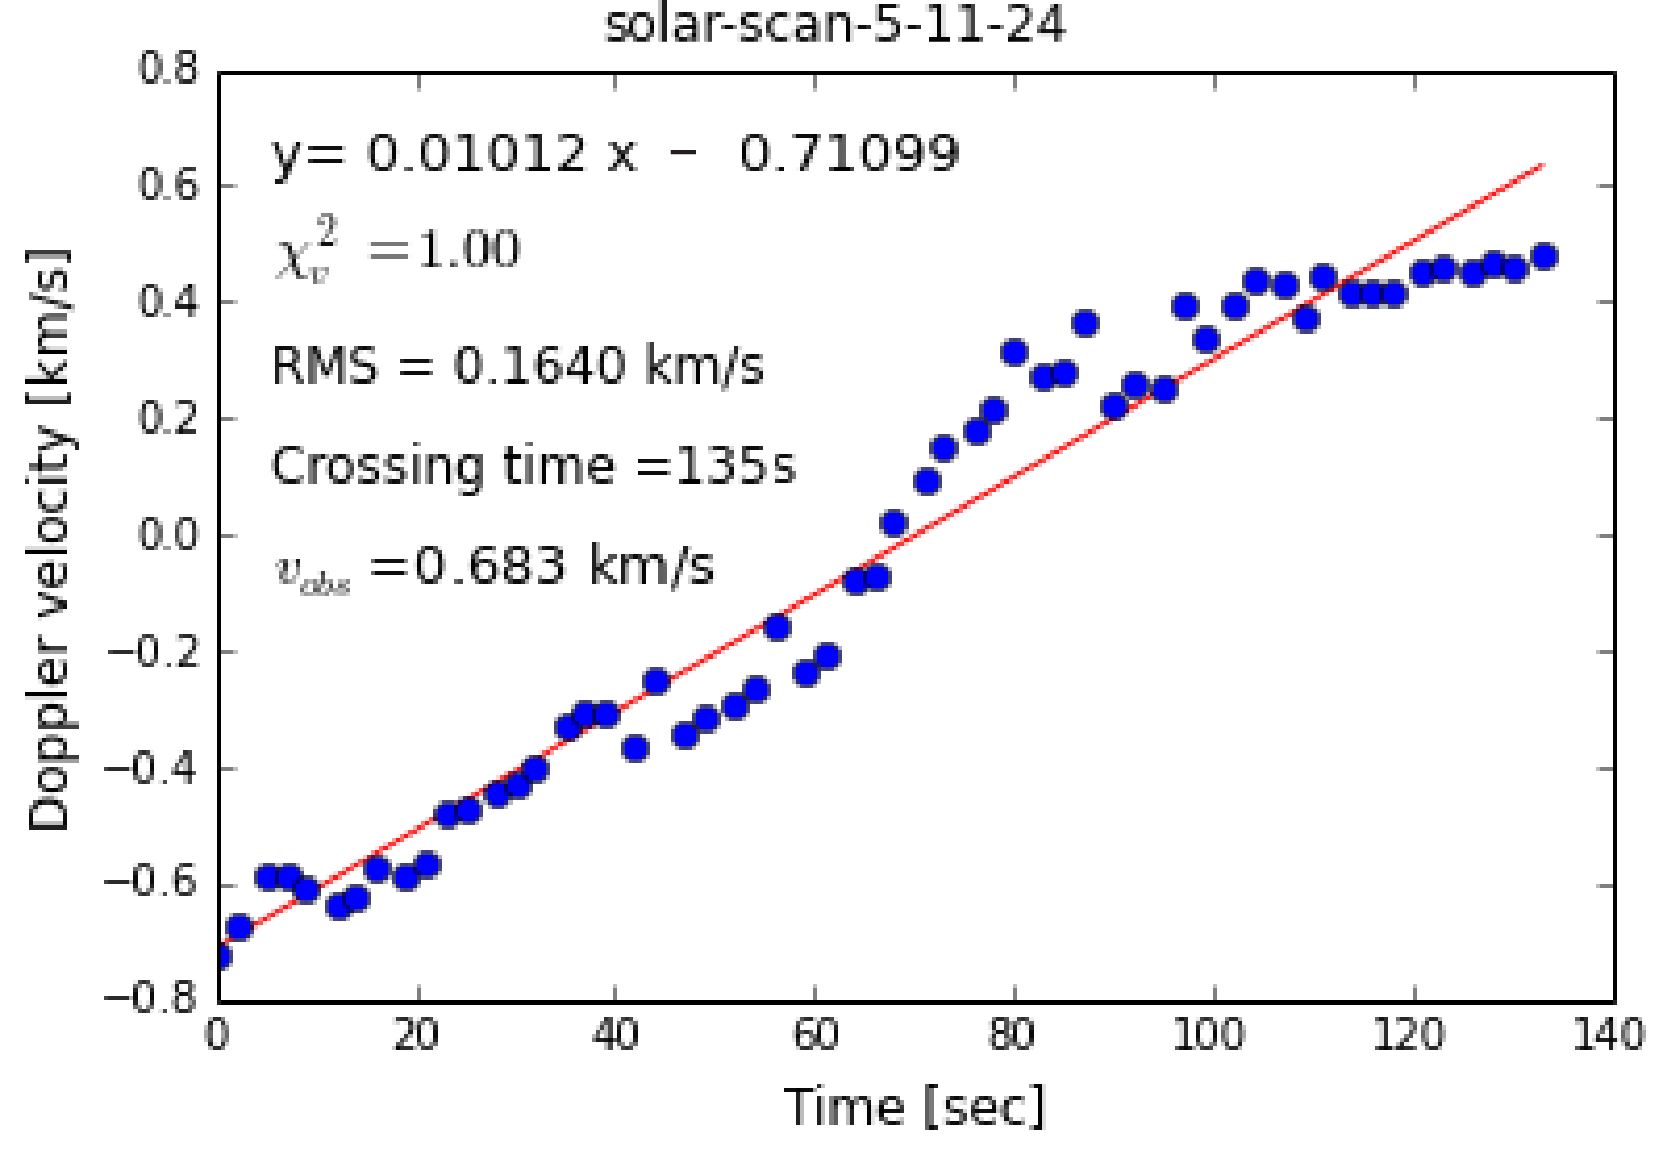
\includegraphics[width=0.5\textwidth]{figures/long_cord_dv}
\caption{}
\label{long_cord_dv}
\end{figure}
\begin{figure}[h!]
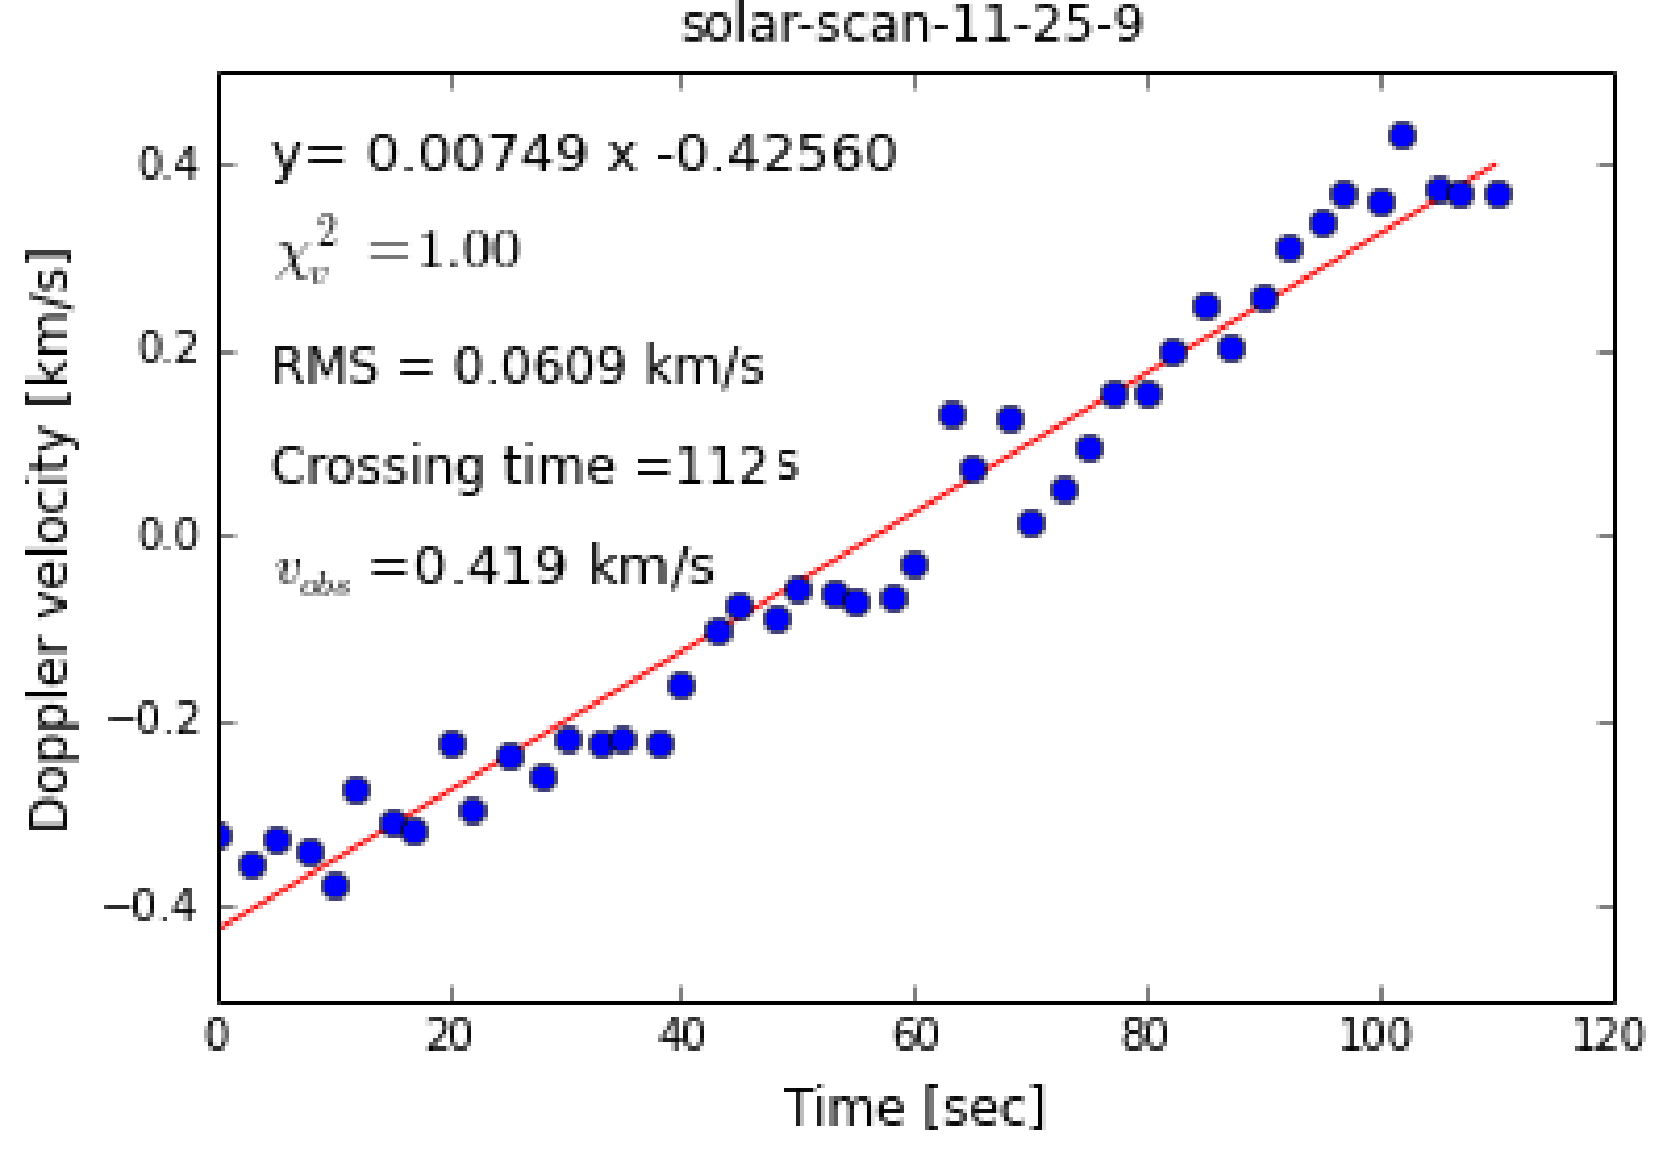
\includegraphics[width=0.5\textwidth]{figures/short_cord_dv}
\caption{}
\label{short_cord_dv}
\end{figure}

\label{results}
Excluding the saturated or partially shaded \footnote{The shading effect could be seen from the decrease in intensity in the middle of the scan in the time series plot, which is clearly not an effect of limb darkening.} solar scans, we conducted this analysis on 8 datasets of the same order. 
\\
Since the crossing time of the scan depends impact parameter of the observer's line of sight, different scans should have the approximately gradient despite the different in the chord cut from  each drift scan. The standard deviation of the all the gradients obtained \footnote{with one outlier removed} is 0.0015 km/$s^2$, which shows that the gradients are fairly constant, with an average value of 0.0118 km/$s^2$. These gradients are used to calculate the observed velocity at the limb of the Sun by multiplying with the half crossing time (i.e. time for drift scan to drift from center to limb)
This procedure, combined with the model fit for crossing time determination, is more statistically robust than simply taking the first and last Doppler velocities of the solar scan, since it is a continuous approximation of the velocity rather than a discrete selection . Also, due to the limbing effect, there are less photons received on the edges. Therefore, the errors on the velocity values measured are larger, which makes it even more unreliable to use the single measurements .
\subsection{Coordinate transformation}
rotational matrix
\begin{equation}
\bBigg@{4}(\begin{matrix}
\cos\xi & 0 &\sin\xi \\ 
0 &1  &0 \\ 
-\sin\xi &0  &\cos\xi 
\end{matrix}\bBigg@{4})
\label{rotmatrix1}
\end{equation}

\begin{equation}
\bBigg@{4}(\begin{matrix}
1& 0 &0 \\ 
0 &\cos\eta  &\sin\eta \\ 
0 &\sin \eta  &\cos\eta 
\end{matrix}\bBigg@{4})
\label{rotmatrix2}
\end{equation}
We obtain the North pole angle($\eta$) and the observer sub-latitudes($\xi$) from the JPL Horizon web interface.
$\eta$ describes tilt of the Sun's axis of rotation and $\xi $----.
By conducting these coordinate transformation on the mean observed velocity calculated in Sec.\ref{results}, we obtain 1.257\rpm 0.0185 km/s for the solar radial velocity.
\subsection{Angular Size of Sun}
\label{size_calc}
\subsection{Error Propagation}
The RMS residual  computed for each scan yields an estimate of how much the datapoints deviates from the model and informs how good the linear fit is.  Using the least squares method on the linear model y=a+bx, we can derive an analytical relation to obtain the slope b as well as the error on the value of the slope as described by Press and Vetterling\footnote{Above equation is an expanded form of  Eq.15.2.9 in the referenced text.}  (1992): 
\begin{equation}
\sigma_b^2 = \frac{\sum\limits_{i=1}^N\frac{1}{\sigma_i^2}}{\sum\limits_{i=1}^N\frac{x_i^2}{\sigma_i^2}\sum\limits_{i=1}^N\frac{1}{\sigma_i^2}-\Big(\sum\limits_{i=1}^N\frac{x_i}{\sigma_i^2}\Big)^2}
\label{ls}
\end{equation}
This value is computed by the a part of the regression algorithm\footnote{\texttt{scipy.stats.linregress}}, the average error on the slope is 0.000276km/$s^2$. The error is propagated when deriving the limb velocity to obtain the value of observed velocity  0.3799 \rpm 0.0185 km/s. (FINISH THIS BY PROPAGTING TO ANGULAR SIZE!)
\section{Conclusion}
In this lab, we conveniently chose to use the 35$^\text{th}$ for wavelength calibration and conduct the doppler velocity determination. In order to obtain a more precise measurement, we can conduct wavelength calibration on other orders to increase the number of spectral lines used for each cross correlation analysis and thereby decreasing the quoted error bar on the measurement.
 \section*{References}
 \begin{footnotesize}
 \begin{itemize}
 \item Carroll, Bradley W., and Dale A. Ostlie. \textit{An Introduction to Modern Astrophysics}. San Francisco: Pearson Addison-Wesley, 2007. Print.
\item Chromey, Frederick R. \textit{To Measure the Sky: An Introduction to Observational Astronomy}. Cambridge: Cambridge UP, 2010. Print.
\item Press, William H., and William T. Vetterling. \textit{Numerical Recipes in C: The Art of Scientific Computing}. Cambridge University Press, 1992.  
\end{itemize}
% \bibliography{references}
%\bibliographystyle{elsarticle-harv}
  \end{footnotesize}

\end{document}
